\section{Results and Analysis}
\label{sec:results-analysis}

This section presents the experimental evidence in the same order in which the benchmark design was developed and validated. The first phase establishes the baseline behavior of the benchmark and verifies the methodological assumptions needed for fair comparison. The second phase provides the main matched grid-level timing evidence across the selected PyTorch CUDA accumulation paths. The third phase complements the timing results with profiler evidence for representative cases, allowing the observed performance differences to be related to the CUDA execution paths used by each API.

The analysis therefore separates three roles. Phase 1 is treated as a calibration and validation phase, because its purpose is to justify the final benchmark protocol rather than to provide the main paper-level performance claim. Phase 2 is treated as the primary timing phase, because it compares the selected operations across a matched workload grid. Phase 3 is treated as the attribution phase, because it explains selected Phase 2 patterns through CUDA profiler evidence. This separation is important because the study does not rely on a single timing table or a single profiler run; instead, the final interpretation combines protocol validation, matched timing, and representative execution-path analysis.

\subsection{Phase 1 Baseline Calibration and Methodological Checks}

Phase 1 was used to establish a reliable benchmark protocol before the final matched comparison was performed. At this stage, the purpose was not to select a final winning API, but to identify which timing scope, workload construction, and validation rules were appropriate for comparing sparse-index accumulation paths during backpropagation-style computation. The early benchmark runs helped separate experimental configurations that were useful for methodological diagnosis from configurations that were suitable for final matched comparison.

A central outcome of this phase was the need to define a fair dense-gradient accumulation scope. For direct accumulation APIs such as \texttt{index\_add} and \texttt{scatter\_add}, timing only the update kernel without accounting for the dense output buffer would not match the practical cost of producing a dense gradient-like result. Phase 1 therefore motivated the final timing scope in which dense output allocation or zero initialization is included where required by the operation design. This made the later comparison closer to the practical cost of producing the accumulated output, rather than measuring only an isolated kernel fragment.

Phase 1 also clarified the role of \texttt{Embedding.backward}. The embedding backward path is not simply a syntactic variant of \texttt{index\_add} or \texttt{scatter\_add}. It is a framework-level backward path with its own internal dispatch behavior and memory-management assumptions. For this reason, the final protocol treats \texttt{Embedding.backward} as a realistic training-related path rather than forcing it into the exact same implementation scope as the direct accumulation APIs. This distinction is important because the paper studies the behavior of standard PyTorch CUDA paths as they are exposed to practitioners, not an artificially rewritten version of each operation.

The first phase further established the importance of correctness validation before timing interpretation. Sparse-index accumulation workloads often contain repeated indices, and different execution paths may accumulate floating-point values in different orders. As a result, bitwise equality is not an appropriate universal requirement for accepting a timing row. Phase 1 therefore motivated the use of tolerance-based numerical validation and the exclusion of failed correctness rows from paired performance claims. This validation gate was then carried forward into the later matched benchmark and profiler phases.

Another methodological result from Phase 1 was the decision to distinguish decisive timing differences from near-ties. Small differences between operation medians can occur because of normal runtime variability, measurement noise, or cache and scheduling effects. Treating every raw minimum as a meaningful winner would overstate the evidence. The later analysis therefore applies a practical margin rule, where a winner is treated as decisive only when the runner-up is more than 5\% slower. Cases below this threshold are retained in the dataset but interpreted as near-ties rather than strong performance evidence.

Phase 1 also informed the workload design used in the final study. The benchmark needed to include not only uniform index distributions, but also skewed patterns such as Zipf and hotspot distributions. These distributions are relevant because duplicate indices and hot rows can change the behavior of accumulation kernels. The preliminary checks therefore motivated a workload design that varies row count, number of indices, feature dimension, distribution type, index ordering, and cache-related conditions. This broader design was necessary to avoid drawing conclusions from a single synthetic shape or a single index distribution.

The outcome of Phase 1 was therefore a calibrated experimental protocol for the final comparison. The final protocol uses matched workloads, correctness-gated rows, median CUDA-event timing, a practical-margin rule for winner classification, and a distinction between grid-level timing evidence and profiler-based attribution. Phase 1 is not presented as the main evidence for the paper's performance claims; instead, it explains why the subsequent Phase 2 and Phase 3 analyses are structured as matched timing and representative profiling phases.

\subsection{Matched Phase 2 Benchmark Results}

The matched Phase 2 benchmark provides the main grid-level evidence for the study. In this phase, the three selected PyTorch accumulation paths were compared under shared workload configurations, using the same rows, index counts, feature dimensions, distribution types, layout settings, and cache conditions within each matched case. The purpose of this phase was to determine whether the fastest API path is stable across environments or whether it changes with the workload and software/hardware stack.

Table~\ref{tab:phase2-winner-counts} summarizes the practical-margin winner counts across the matched Phase 2 grid. The local GTX1650Ti environment favored \texttt{embedding} most often, with 96 decisive wins out of 162 matched configurations. The same environment selected \texttt{index\_add} in 60 configurations, while \texttt{scatter\_add} did not obtain a decisive win under the practical-margin rule. Six configurations were classified as ties. In contrast, the T4 environment favored \texttt{scatter\_add} most often, with 92 decisive wins out of 162 configurations. The repeated T4 run reproduced the same qualitative pattern, with \texttt{scatter\_add} selected in 93 out of 162 configurations.

% Source summary: sparse-gradient/phase2_analysis_v2/ and matched Phase 2 analysis.
\begin{table}[tbp]
\centering
\small
\caption{Matched Phase 2 winner counts for the three primary accumulation paths under the 5\% practical-margin rule.}
\label{tab:phase2-winner-counts}
\resizebox{\linewidth}{!}{%
\begin{tabular}{lrrrrrr}
\toprule
Environment & \texttt{index\_add} & \texttt{scatter\_add} & \texttt{embedding} & Tie & Total matched configurations & Most frequent decisive API \\
\midrule
GTX1650Ti & 60 & 0 & 96 & 6 & 162 & \texttt{embedding} \\
T4 & 5 & 92 & 25 & 40 & 162 & \texttt{scatter\_add} \\
T4\_repeat & 1 & 93 & 27 & 41 & 162 & \texttt{scatter\_add} \\
\bottomrule
\end{tabular}
}%
\end{table}


The Phase 2 results therefore indicate that there is no single universally dominant API path across the studied environments. The local stack most often favors the embedding backward path, whereas the T4 stacks most often favor the scatter-add path. This difference is not interpreted as an isolated GPU-hardware effect, because the environments differ in GPU model, operating system, PyTorch version, CUDA version, and hosted execution conditions. Instead, the result motivates a stack-level interpretation: the relative cost of the available PyTorch CUDA paths depends on the combination of workload structure and execution environment.

The practical-margin rule is important for interpreting these counts. Configurations in which the fastest and runner-up operations differ by less than the selected 5\% threshold are retained as near-ties rather than treated as decisive evidence. This prevents small timing differences from being overinterpreted as meaningful API-level superiority. Consequently, the Phase 2 result should be read as a matched practical-performance characterization, not as a statistical proof of universal API ranking.

\subsection{Representative Phase 3 Profiling Results}

Phase 3 complements the Phase 2 timing grid by profiling a representative subset of six workload cases. The purpose of this phase is not to replace the broader timing evidence, but to inspect the CUDA execution paths associated with the selected PyTorch APIs. Each representative case is evaluated for \texttt{index\_add}, \texttt{scatter\_add}, and \texttt{Embedding.backward}, resulting in 18 profiled case-operation rows per environment.

The profiling outputs passed the basic execution and correctness checks in both environments. Each environment produced 18 successful case-operation rows, with no failed execution status and no correctness failures. CUDA kernel attribution was available for all 18 profiled rows in both environments. The T4 environment contained one host-overhead warning, associated with the \texttt{embedding} operation in case04; this case is therefore interpreted cautiously when making GPU-clean attribution claims.

Fig.~\ref{fig:phase3-median-ms} shows the representative Phase 3 event-timing medians by case and operation. These values are useful for relating the profiled subset to the broader timing behavior, but they are not treated as a replacement for the matched Phase 2 grid. The profiled subset uses a smaller number of cases and is primarily designed for attribution rather than grid-level performance counting.

\begin{figure}[tbp]
\centering
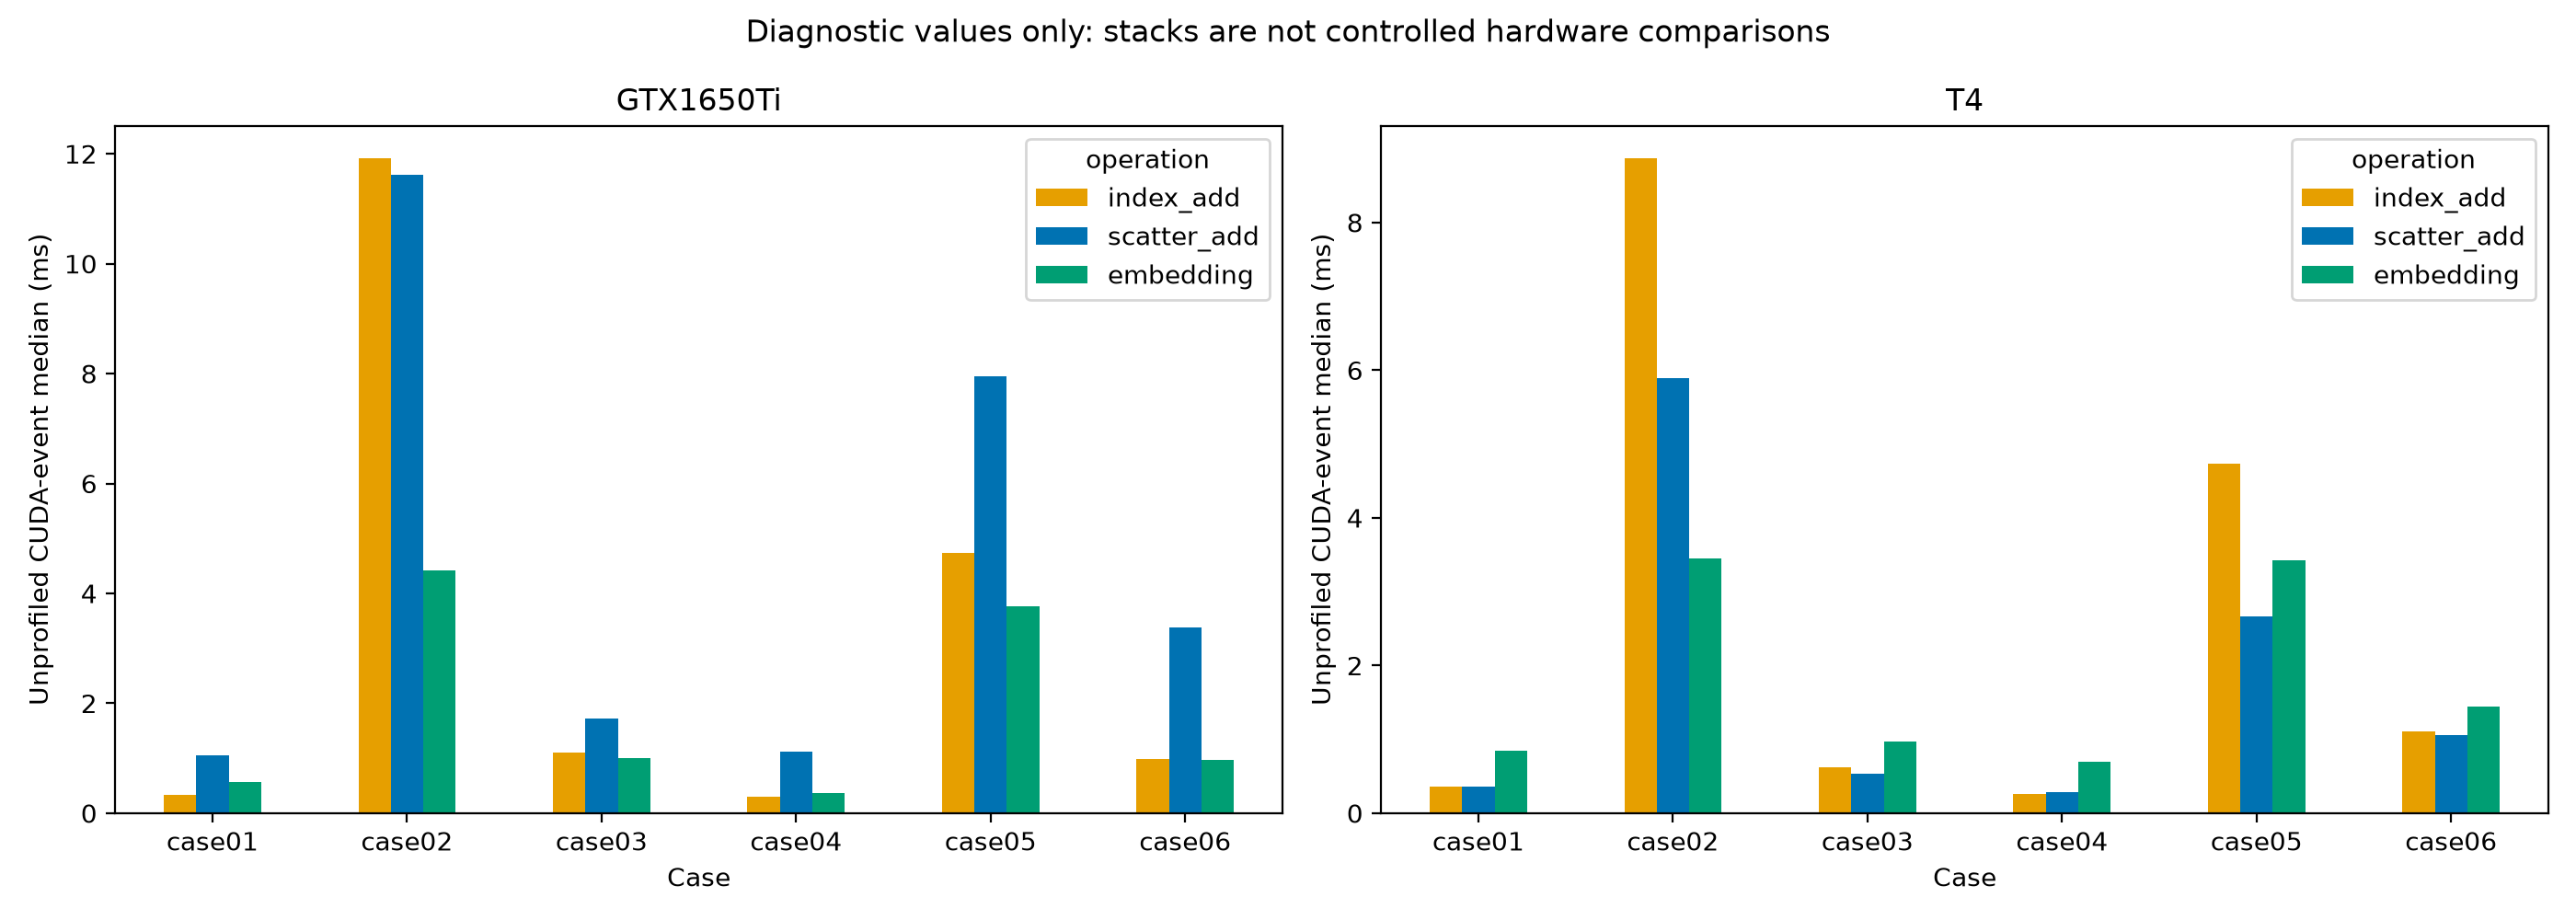
\includegraphics[width=0.80\linewidth]{figures/phase3_median_ms_by_case_operation.png}
\caption{Phase 3 median CUDA-event timing by representative case and operation. These timings describe the profiled subset and are interpreted together with the broader matched Phase 2 grid.}
\label{fig:phase3-median-ms}
\end{figure}

Fig.~\ref{fig:phase3-gpu-busy} summarizes the profiler-derived GPU-busy proxy. The proxy is used only as a warning signal for possible host overhead, not as a hardware utilization counter. Most profiled case-operation rows have high proxy values, supporting their use for execution-path attribution. The main exception is the T4 \texttt{embedding} row in case04, which is flagged and therefore not used as a clean GPU-bound claim.

\begin{figure}[tbp]
\centering
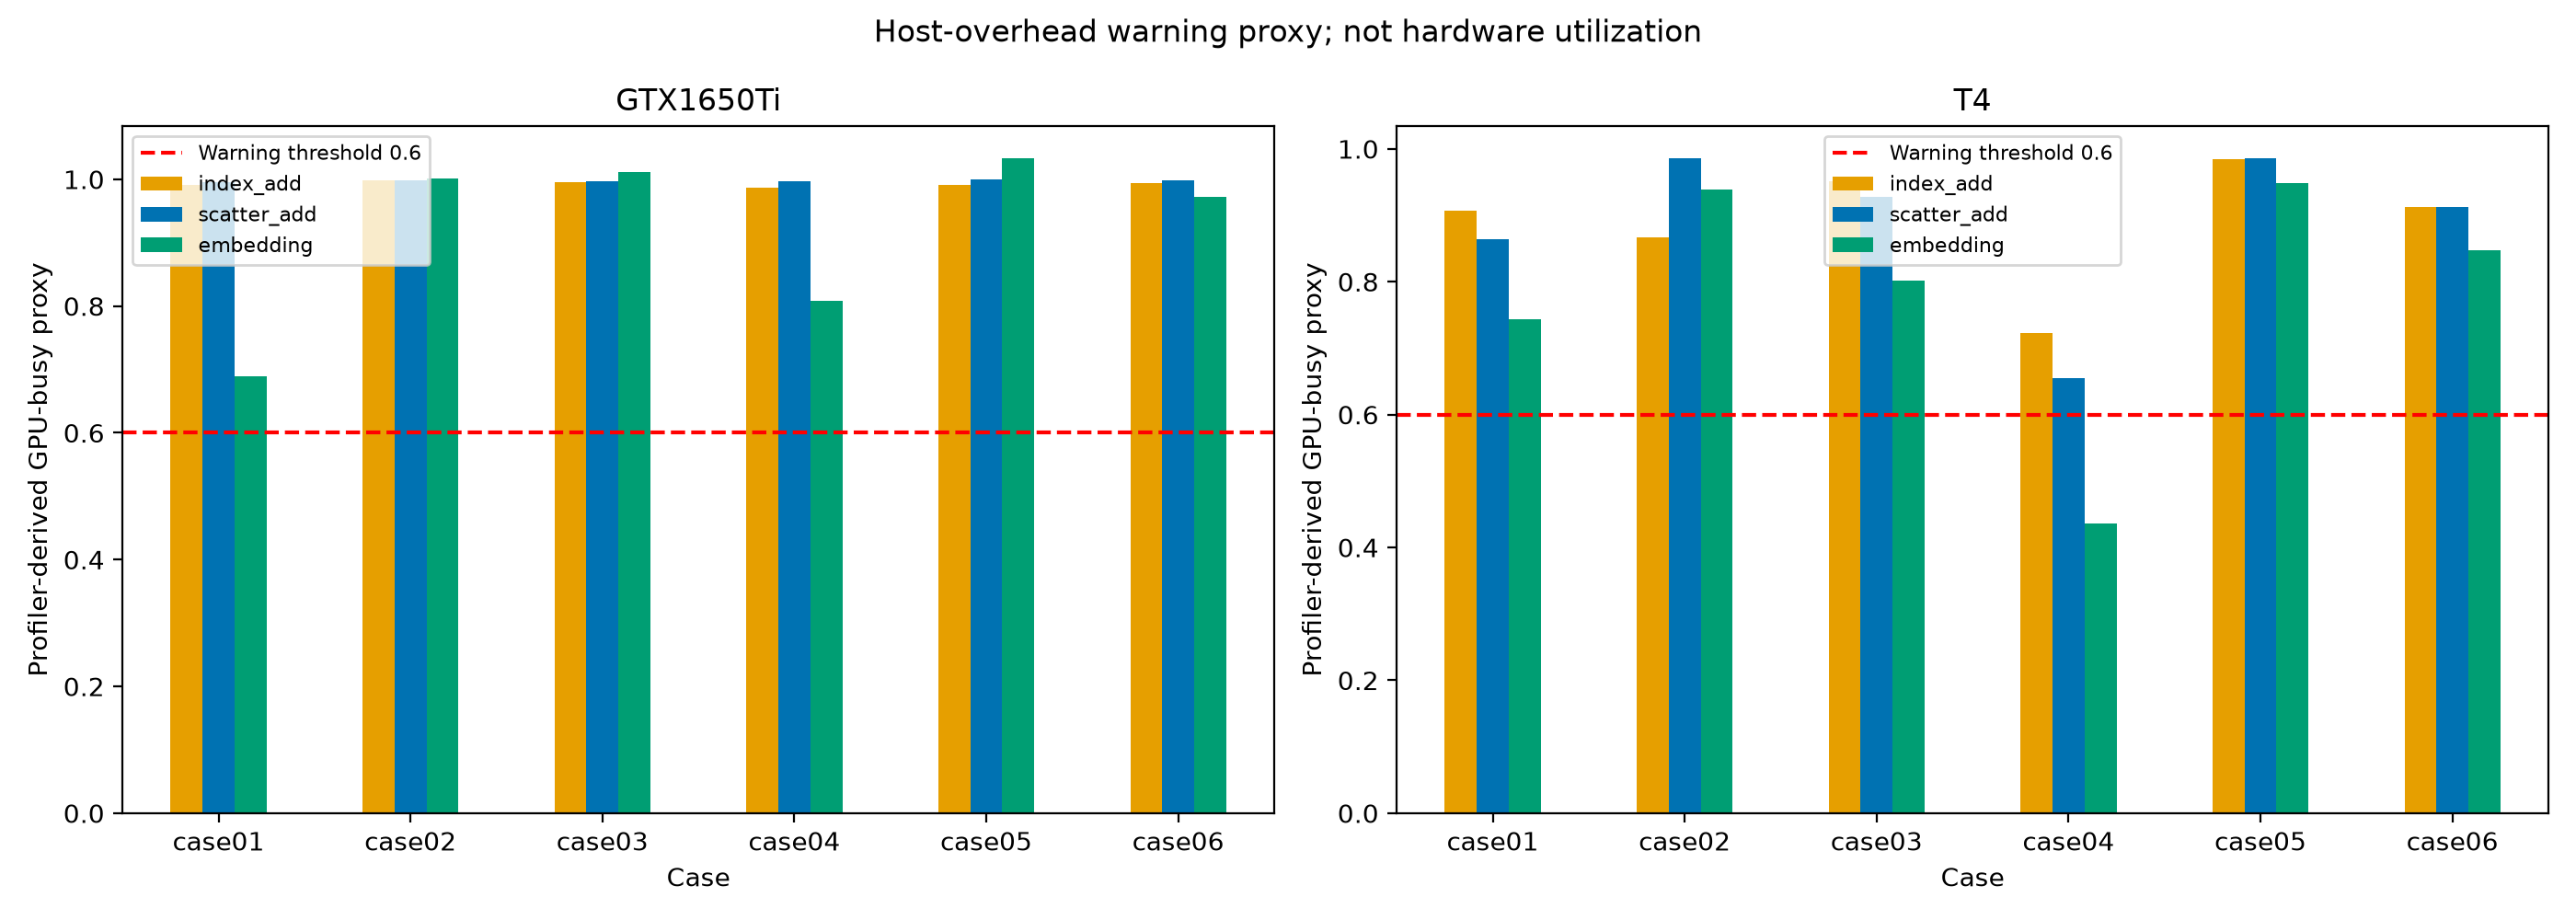
\includegraphics[width=0.80\linewidth]{figures/phase3_gpu_busy_fraction_by_case_operation.png}
\caption{Profiler-derived GPU-busy proxy by representative case and operation. The proxy is diagnostic only and is not interpreted as hardware utilization.}
\label{fig:phase3-gpu-busy}
\end{figure}

The kernel-category summary in Table~\ref{tab:phase3-kernel-category-summary} and Fig.~\ref{fig:phase3-kernel-category-share} shows that the three API paths are not merely different syntactic forms of the same CUDA behavior. The \texttt{index\_add} path is dominated by indexed accumulation kernels, the \texttt{scatter\_add} path is dominated by scatter/gather-style accumulation kernels, and the embedding backward path uses a multi-kernel composition that includes accumulation as well as sorting, scanning, or uniqueness-related components.

% Source summary: sparse-gradient/phase3_comparison_v2/phase3_kernel_category_summary.csv.
% Detailed per-case rows can be moved to an appendix or supplementary material later.
\begin{table}[tbp]
\centering
\small
\caption{Mean CUDA kernel-category shares for the representative Phase 3 profiles. Shares are averaged across the profiled cases for each environment and operation.}
\label{tab:phase3-kernel-category-summary}
\resizebox{\linewidth}{!}{%
\begin{tabular}{lllrrr}
\toprule
Environment & Operation & Dominant category & Dominant share & Secondary category & Secondary share & Other share \\
\midrule
GTX1650Ti & embedding & \texttt{embedding\_accumulate} & 0.8271 & \texttt{sort\_scan\_unique} & 0.1217 & -- \\
GTX1650Ti & \texttt{index\_add} & \texttt{index\_add\_accumulate} & 0.9677 & \texttt{zero\_fill\_memset} & 0.0323 & -- \\
GTX1650Ti & \texttt{scatter\_add} & \texttt{scatter\_add\_accumulate} & 0.9817 & \texttt{zero\_fill\_memset} & 0.0183 & -- \\
T4 & embedding & \texttt{embedding\_accumulate} & 0.6697 & \texttt{sort\_scan\_unique} & 0.2342 & 0.0347 \\
T4 & \texttt{index\_add} & \texttt{index\_add\_accumulate} & 0.9647 & \texttt{zero\_fill\_memset} & 0.0353 & -- \\
T4 & \texttt{scatter\_add} & \texttt{scatter\_add\_accumulate} & 0.9518 & \texttt{zero\_fill\_memset} & 0.0482 & -- \\
\bottomrule
\end{tabular}
}%
\end{table}


\begin{figure}[tbp]
\centering
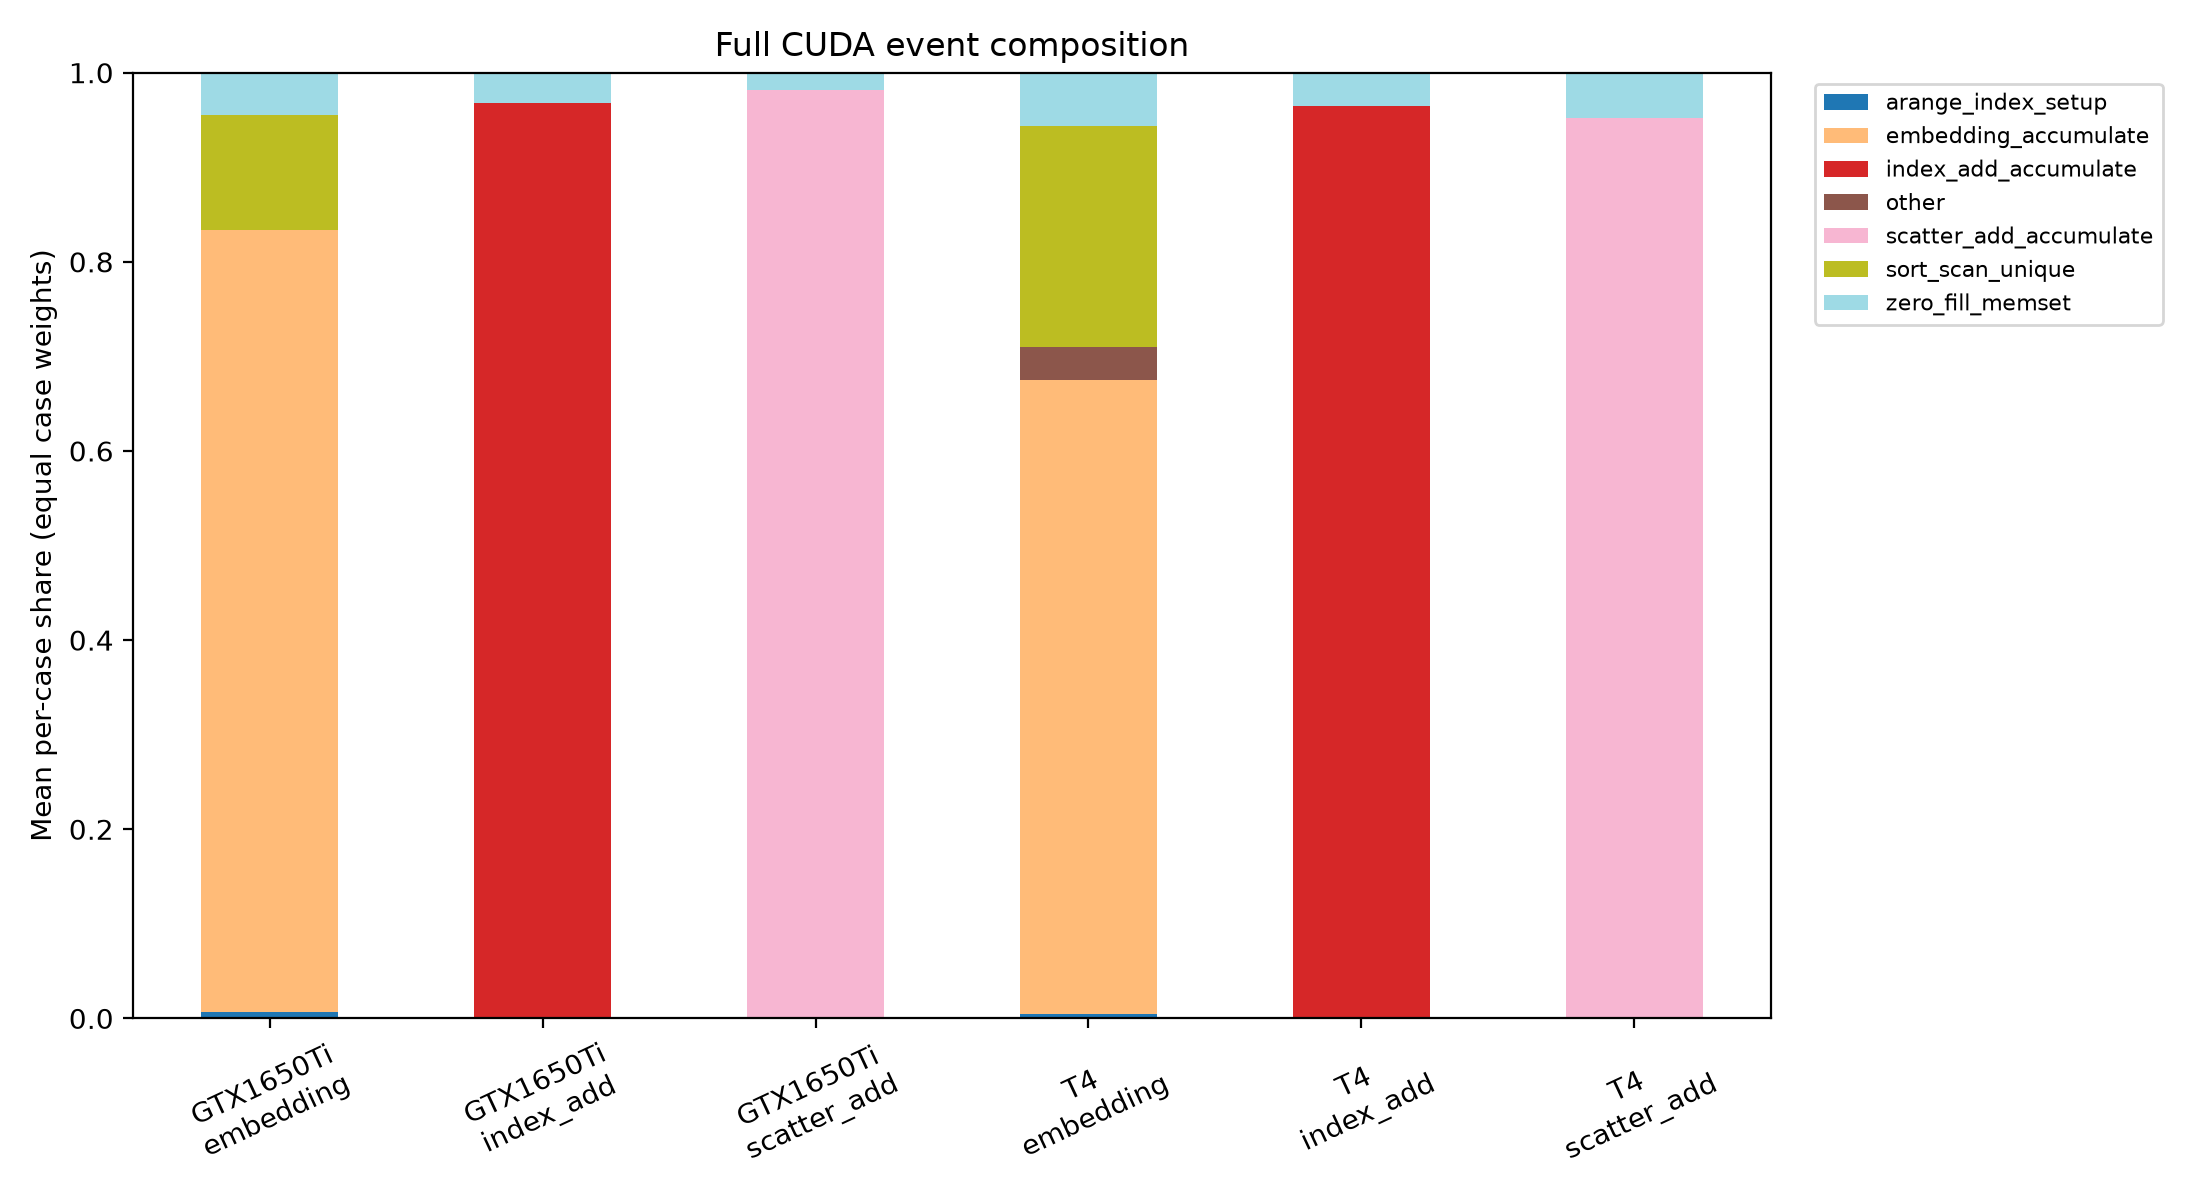
\includegraphics[width=0.80\linewidth]{figures/phase3_kernel_category_share.png}
\caption{Mean CUDA kernel-category share for the representative Phase 3 profiles. Category shares are computed from CUDA device events and summarize observed execution-path composition.}
\label{fig:phase3-kernel-category-share}
\end{figure}

The mean category shares support the intended execution-path interpretation. In both environments, \texttt{index\_add} is dominated by the \texttt{index\_add\_accumulate} category, while \texttt{scatter\_add} is dominated by the \texttt{scatter\_add\_accumulate} category. The embedding backward path is dominated by \texttt{embedding\_accumulate}, but it also contains a non-trivial \texttt{sort\_scan\_unique} component. The \texttt{other} category remains below the selected control threshold, which reduces the risk that the main attribution is hiding a large unclassified portion of CUDA time.

\subsection{Case-Level Cross-Environment Comparison}

The Phase 3 case-level comparison links the representative profiling subset to both environments and to the broader Phase 2 grid. Table~\ref{tab:phase3-case-comparison} summarizes the raw case-level winners, margins, and winner-relation categories for the six representative cases.

% Source: ../sparse-gradient/phase3_comparison_v2/phase3_case_comparison.csv
\begin{table}[tbp]
\centering
\small
\caption{Phase 3 case-level comparison across environments.}
\label{tab:phase3-case-comparison}
\resizebox{\linewidth}{!}{%
\begin{tabular}{lrrrrl}
\toprule
Case & Local winner & T4 winner & Local margin & T4 margin & Winner relation \\
\midrule
case01 & index\_add & scatter\_add & 1.670 & 1.022 & reversal near-tie \\
case02 & embedding & embedding & 2.631 & 1.706 & same decisive \\
case03 & embedding & scatter\_add & 1.116 & 1.186 & reversal decisive \\
case04 & index\_add & index\_add & 1.197 & 1.058 & same decisive \\
case05 & embedding & scatter\_add & 1.257 & 1.285 & reversal decisive \\
case06 & embedding & scatter\_add & 1.015 & 1.040 & reversal near-tie \\
\bottomrule
\end{tabular}
}%
\end{table}

Two cases provide the strongest evidence of a cross-environment reversal. In case03, the local GTX1650Ti stack selects \texttt{embedding} decisively, while the T4 stack selects \texttt{scatter\_add} decisively. In case05, the same pattern appears again: the local stack selects \texttt{embedding}, whereas the T4 stack selects \texttt{scatter\_add}. Both cases pass the stronger clean-reversal gates in the comparison analysis: they are decisively separated, have clean GPU-busy proxy status, and use exact index pairing across environments.

Fig.~\ref{fig:phase3-case-winner-comparison} visualizes the case-level winner comparison. The figure highlights that the representative subset does not support a universal ordering of APIs. Instead, it shows a mixture of agreement, near-ties, and decisive reversals.

\begin{figure}[tbp]
\centering
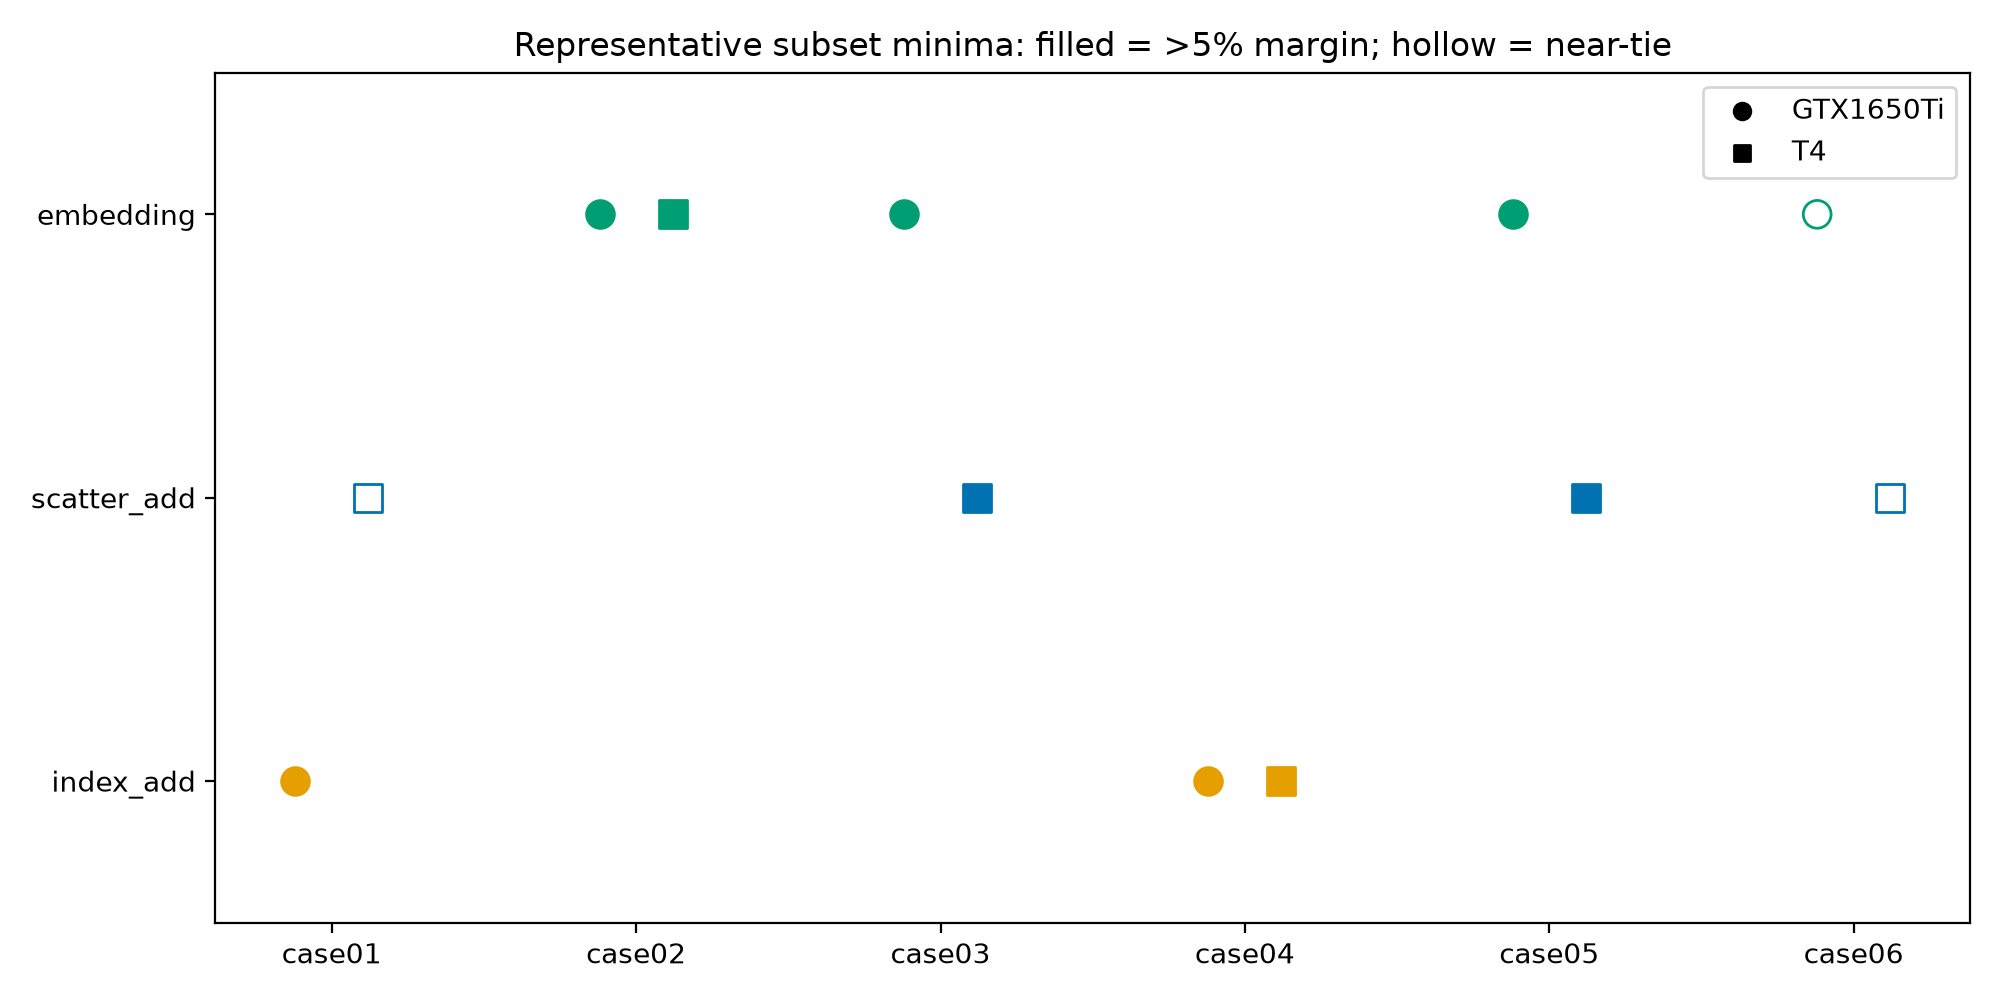
\includegraphics[width=0.80\linewidth]{figures/phase3_case_winner_comparison.png}
\caption{Representative Phase 3 winner comparison across environments. Filled markers indicate decisive practical-margin winners, while near-ties are interpreted as weak evidence.}
\label{fig:phase3-case-winner-comparison}
\end{figure}

The remaining cases serve as controls or cautionary examples. In case02, both environments select \texttt{embedding} decisively. In case04, both environments select \texttt{index\_add} decisively, although the T4 \texttt{embedding} row has a host-overhead warning and therefore prevents a fully GPU-clean claim for that case. Cases case01 and case06 exhibit different raw winners across environments, but at least one side is a near-tie, so these cases are treated as weak evidence rather than decisive reversals.

Table~\ref{tab:phase3-phase2-case-join} links the six representative Phase 3 cases back to the broader Phase 2 grid. This join is important because it verifies that the representative profiling cases are not disconnected from the main timing study. All six representative cases are present in the Phase 2 grid. The strongest reversal cases, case03 and case05, agree with the Phase 2 margin-aware winners in both environments: the local stack favors \texttt{embedding}, and the T4 stack favors \texttt{scatter\_add}. This supports the interpretation that these two profiled cases are representative examples of the broader environment-dependent behavior observed in Phase 2.

% Source: ../sparse-gradient/phase3_comparison_v2/phase3_phase2_case_join.csv
\begin{table}[tbp]
\centering
\small
\caption{Matched Phase 2 and Phase 3 case winners.}
\label{tab:phase3-phase2-case-join}
\resizebox{\linewidth}{!}{%
\begin{tabular}{lllllll}
\toprule
Case & Phase 2 local & Phase 2 T4 & Phase 2 T4 repeat & Local agree & T4 agree & Phase 3 local/T4 \\
\midrule
case01 & index\_add & tie & tie & True & False & index\_add / scatter\_add \\
case02 & embedding & embedding & embedding & True & True & embedding / embedding \\
case03 & embedding & scatter\_add & scatter\_add & True & True & embedding / scatter\_add \\
case04 & index\_add & tie & tie & True & False & index\_add / index\_add \\
case05 & embedding & scatter\_add & scatter\_add & True & True & embedding / scatter\_add \\
case06 & tie & index\_add & tie & False & False & embedding / scatter\_add \\
\bottomrule
\end{tabular}
}%
\end{table}

The case-level evidence therefore reinforces the grid-level result without replacing it. Phase 2 establishes the broader matched-performance pattern, while Phase 3 explains selected cases in terms of execution-path differences. The combination of the two phases is stronger than either alone: the timing grid shows that the fastest API changes across environments, and the profiler shows that the compared APIs exercise distinct CUDA paths.

\subsection{CUDA Path Attribution}

The claim-check table summarizes the evidence gates used to decide which result-level statements are supported by the data. These gates are included to avoid overclaiming from the representative profiling subset.

\begin{table}[tbp]
\centering
\scriptsize
\caption{Evidence gates used to avoid overclaiming from the representative Phase 3 profiling subset.}
\label{tab:phase3-claim-checks}
\resizebox{\linewidth}{!}{%
\begin{tabular}{lll}
\toprule
Check & Status & Evidence \\
\midrule
index\_add path dominance & Pass & GTX1650Ti=0.9677; T4=0.9647 \\
scatter\_add path dominance & Pass & GTX1650Ti=0.9817; T4=0.9518 \\
embedding accumulation present & Pass & GTX1650Ti=0.8271; T4=0.6697 \\
embedding sort/scan present & Pass & GTX1650Ti=0.1217; T4=0.2342 \\
other share controlled & Pass & T4/embedding=0.0347 \\
environment difference present & Pass & GTX=embedding; T4=scatter\_add \\
representative reversals present & Pass & case03, case05 \\
\bottomrule
\end{tabular}
}%
\end{table}


The path-dominance checks pass for both direct accumulation APIs. The \texttt{index\_add} path is dominated by the \texttt{index\_add\_accumulate} category in both environments, and the \texttt{scatter\_add} path is dominated by the \texttt{scatter\_add\_accumulate} category in both environments. This supports the claim that the two APIs dispatch to distinct CUDA reduction paths under the profiled workloads.

The embedding checks also pass. The embedding backward path contains a dominant accumulation component, but it also includes sorting, scanning, or uniqueness-related work. This distinguishes \texttt{Embedding.backward} from the direct \texttt{index\_add} and \texttt{scatter\_add} paths. The result is consistent with the interpretation that embedding backward is a specialized framework path rather than a simple alias for either direct accumulation API.

The claim checks also confirm that the broader Phase 2 environment-dependent pattern is present and that the representative Phase 3 subset contains strong clean reversals. In particular, case03 and case05 satisfy the strict evidence conditions: they are decisive reversals, they are not host-warning cases, they have stable timing evidence, and they use exact index pairing. These cases therefore support the paper-level statement that the relative cost of sparse-index accumulation paths can change with workload and software/hardware stack.

At the same time, the attribution remains conservative. The kernel categories are based on profiler event names and CUDA event durations, not on low-level hardware counters. Therefore, they describe observed execution paths but do not prove microarchitectural causality. The evidence supports an API-path and stack-level interpretation, not a claim that one GPU architecture alone causes the observed differences.

\subsection{Result-Level Discussion}

The combined results answer the central question of the study: standard PyTorch CUDA APIs that express related sparse-index accumulation behavior do not necessarily have interchangeable performance characteristics during backpropagation-style workloads. In the matched Phase 2 grid, the local GTX1650Ti stack most often favors the embedding backward path, whereas the T4 stacks most often favor \texttt{scatter\_add}. In the representative Phase 3 profiles, the strongest reversal cases show the same pattern at the case level: local execution favors \texttt{embedding}, while T4 execution favors \texttt{scatter\_add}.

The results also show why the difference should not be reduced to a simple API ranking. Some representative cases agree across environments, some differ only as near-ties, and two cases provide strong decisive reversals. This mixed behavior indicates that the best operation depends on workload shape, index distribution, duplicate structure, and the software/hardware stack. A recommendation such as ``always use \texttt{scatter\_add}'' or ``always use \texttt{Embedding.backward}'' would not be supported by the evidence.

The execution-path attribution provides a practical explanation for this behavior. Although the operations represent related accumulation-style computations, they dispatch to different CUDA paths. \texttt{index\_add} and \texttt{scatter\_add} use different direct accumulation kernels, while \texttt{Embedding.backward} uses a multi-kernel path that includes embedding-specific accumulation and sorting or segmentation-related work. These differences create opportunities for the relative cost of the APIs to change when the workload or execution stack changes.

For practitioners, the results suggest that sparse-gradient accumulation paths in AI training should not be selected purely from high-level API semantics. When sparse-index accumulation is a relevant part of the backward pass, especially in embedding-heavy models, recommender workloads, or other skewed-index settings, the actual execution path and target environment can materially affect performance. Microbenchmarking and profiler inspection remain useful tools for identifying which API path is most appropriate for a specific workload and deployment stack.

Finally, the results define the boundary of the present evidence. The study characterizes controlled sparse-index accumulation workloads and representative profiler cases; it does not measure full model training throughput, convergence behavior, distributed execution, or custom CUDA alternatives. Therefore, the contribution is best understood as a controlled characterization of PyTorch CUDA sparse-index gradient accumulation paths during backpropagation-style computation, rather than as a complete benchmark of AI training systems.